\documentclass{beamer}
\mode<presentation>
\usepackage{amsmath}
\usepackage{amssymb}
%\usepackage{advdate}
\usepackage{adjustbox}
\usepackage{subcaption}
\usepackage{enumitem}
\usepackage{multicol}
\usepackage{mathtools}
\usepackage{listings}
\usepackage{float}
\usepackage{graphicx}
\usepackage{url}
\def\UrlBreaks{\do\/\do-}
\usetheme{Boadilla}
\usecolortheme{lily}
\setbeamertemplate{footline}
{
  \leavevmode%
  \hbox{%
  \begin{beamercolorbox}[wd=\paperwidth,ht=2.25ex,dp=1ex,right]{author in head/foot}%
    \insertframenumber{} / \inserttotalframenumber\hspace*{2ex} 
  \end{beamercolorbox}}%
  \vskip0pt%
}
\setbeamertemplate{navigation symbols}{}

\providecommand{\nCr}[2]{\,^{#1}C_{#2}} % nCr
\providecommand{\nPr}[2]{\,^{#1}P_{#2}} % nPr
\providecommand{\mbf}{\mathbf}
\providecommand{\pr}[1]{\ensuremath{\Pr\left(#1\right)}}
\providecommand{\qfunc}[1]{\ensuremath{Q\left(#1\right)}}
\providecommand{\sbrak}[1]{\ensuremath{{}\left[#1\right]}}
\providecommand{\lsbrak}[1]{\ensuremath{{}\left[#1\right.}}
\providecommand{\rsbrak}[1]{\ensuremath{{}\left.#1\right]}}
\providecommand{\brak}[1]{\ensuremath{\left(#1\right)}}
\providecommand{\lbrak}[1]{\ensuremath{\left(#1\right.}}
\providecommand{\rbrak}[1]{\ensuremath{\left.#1\right)}}
\providecommand{\cbrak}[1]{\ensuremath{\left\{#1\right\}}}
\providecommand{\lcbrak}[1]{\ensuremath{\left\{#1\right.}}
\providecommand{\rcbrak}[1]{\ensuremath{\left.#1\right\}}}
\theoremstyle{remark}
\newtheorem{rem}{Remark}
\newcommand{\sgn}{\mathop{\mathrm{sgn}}}
\providecommand{\abs}[1]{\left\vert#1\right\vert}
\providecommand{\res}[1]{\Res\displaylimits_{#1}} 
\providecommand{\norm}[1]{\lVert#1\rVert}
\providecommand{\mtx}[1]{\mathbf{#1}}
\providecommand{\mean}[1]{E\left[ #1 \right]}
\providecommand{\fourier}{\overset{\mathcal{F}}{ \rightleftharpoons}}
%\providecommand{\hilbert}{\overset{\mathcal{H}}{ \rightleftharpoons}}
\providecommand{\system}{\overset{\mathcal{H}}{ \longleftrightarrow}}
	%\newcommand{\solution}[2]{\textbf{Solution:}{#1}}
%\newcommand{\solution}{\noindent \textbf{Solution: }}
\providecommand{\dec}[2]{\ensuremath{\overset{#1}{\underset{#2}{\gtrless}}}}
\newcommand{\myvec}[1]{\ensuremath{\begin{pmatrix}#1\end{pmatrix}}}
\let\vec\mathbf

\lstset{
language=C,
frame=single, 
breaklines=true,
columns=fullflexible
}

\numberwithin{equation}{section}

\title{Presentation - Matgeo}
\author{Aryansingh Sonaye \\
AI25BTECH11032 \\
EE1030 - Matrix Theory}

\date{\today} 
\begin{document}

\begin{frame}
\titlepage
\end{frame}

\section{Problem}
\begin{frame}
\frametitle{Problem Statement}
\textbf{Problem Statement}

\textbf{Problem 4.13.101.} Let $p, q$ amd $r$ be nonzero real numbers that are the $10^{th}, 100^{th}$ and $1000^{th}$ terms of a harmonic progression, respectively. Consider the following system of linear equations

\begin{align}
x + y + z &= 1 \\
10x + 100y + 1000z &= 0 \\
qrx + pry + pqz &= 0
\end{align}

(I) If $\dfrac{q}{r} = 10$, then the system of linear equations has\\
(II) If $\dfrac{p}{r} \neq 100$, then the system of linear equations has\\
(III) If $\dfrac{p}{q} \neq 10$, then the system of linear equations has\\
(IV) If $\dfrac{p}{q} = 10$, then the system of linear equations has

\end{frame}

\section{Problem}
\begin{frame}
\frametitle{Problem Statement}

(A) $x = 0,\; y = \dfrac{10}{9},\; z = -\dfrac{1}{9}$ as a solution\\
(B) $x = \dfrac{10}{9},\; y = -\dfrac{1}{9},\; z = 0$ as a solution\\
(C) infinitely many solutions\\
(D) no solution\\
(E) at least one solution

\end{frame}

\section{Solution}
\subsection{Description of Variables used}
\begin{frame}
\frametitle{Description of Variables used}
\textbf{Input Data}

\begin{table}[H]
\centering
\begin{tabular}{|l |l|}
\hline
Given scalars: & \(p,\; q,\; r\) \\
\hline
HP relation (reciprocals in AP): & $\dfrac{1}{p}=a+9d,\; \dfrac{1}{q}=a+99d,\;$\\ & $\dfrac{1}{r}=a+999d$ \\
\hline
Coefficient matrix (M) rows: & $\vec R_1$=\myvec{1,1,1}, $\vec R_2$=\myvec{10,100,1000},\\ &$\vec R_3$=\myvec{qr,pr,pq} \\
\hline
RHS vector: & $\vec{b}$=\myvec{1\\0\\0}\\
\hline
\end{tabular}
\caption{Input data (scalars and vectors) derived from problem statement}
\label{}
\end{table}


\end{frame}

\subsection{Theoretical Solution }
\begin{frame}
\frametitle{Theoretical Solution}

Given system of equations is:

$\vec{x}$ = 
\myvec{
x \\ y \\ z
}.


% matrix equation

\myvec{
1 & 1 & 1 \\
10 & 100 & 1000 \\
qr & pr & pq
} $\vec{x}$
=
\myvec{
1 \\ 0 \\ 0
}.

\end{frame}

\begin{frame}
\frametitle{Theoretical Solution}


\noindent\textbf{From the system of equations, the augmented matrix formed is:}

\begin{align}
[\,\myvec{M}\mid \vec b\,]
&= \myvec{1 & 1 & 1 & 1 \\
10 & 100 & 1000 & 0 \\
qr & pr & pq & 0}
\end{align}

Eliminate first-column below row1: do \(R_2\leftarrow R_2-10R_1\) and \(R_3\leftarrow R_3-(qr)R_1\):
\begin{align}
\myvec{1 & 1 & 1 & 1 \\
10 & 100 & 1000 & 0 \\
qr & pr & pq & 0}
&\xrightarrow{R_2-10R_1,\;R_3-qrR_1}
\myvec{1 & 1 & 1 & 1 \\
0 & 90 & 990 & -10 \\
0 & pr-qr & pq-qr & -qr}
\end{align}

\end{frame}

\begin{frame}
\frametitle{Theoretical Solution}
Now eliminate the (3,2) entry using row2. Set
\begin{align}
s &= \frac{pr-qr}{90},
\end{align}
and do \(R_3\leftarrow R_3 - sR_2\). Compute the new third-row entries explicitly:

\begin{align}
(3,3)\text{: }&\quad (pq-qr) - s\cdot 990
\\
&= pq-qr - 990\cdot\frac{pr-qr}{90}
\\
&= pq-qr - 11(pr-qr)
\\
&= pq - 11\,pr + 10\,qr \;:=\; D,
\end{align}

\end{frame}

\begin{frame}
\frametitle{Theoretical Solution}
\begin{align}
(3,4)\text{: }&\quad -qr - s(-10)
\\
&= -qr + 10\cdot\frac{pr-qr}{90}
\\
&= -qr + \frac{pr-qr}{9}
\\
&= \frac{pr - 10\,qr}{9} \;:=\; E.
\end{align}

Thus the matrix in row-echelon form is
\begin{align}
[\,\myvec{M}\mid \vec b\,] =
\myvec{1 & 1 & 1 & 1 \\
0 & 90 & 990 & -10 \\
0 & 0 & D & E},
\end{align}
with
\begin{align}
D &= pq - 11\,pr + 10\,qr, \qquad E = \frac{pr - 10\,qr}{9}.
\end{align}

\end{frame}

\begin{frame}
\frametitle{Theoretical Solution}
Conclusions from the echelon form (standard linear algebra facts):
\begin{align}
&\text{If } D\neq 0,\ \text{the system has a unique solution.} \notag \\
&\text{If } D=0 \text{ but } E\neq 0,\ \text{the system is inconsistent (no solution).} \notag \\
&\text{If } D=0 \text{ and } E=0,\ \text{the system has infinitely many solutions (rank 2).} \notag
\end{align}


\noindent\textbf{Using the HP condition,}

Because \(p,q,r\) are the \(10^{\text{th}},100^{\text{th}},1000^{\text{th}}\) terms of an HP,
\begin{align}
\frac{1}{p}=a+9d,\qquad \frac{1}{q}=a+99d,\qquad \frac{1}{r}=a+999d
\end{align}
for some real \(a,d\). Evaluate \(D/(pqr)\) to simplify algebra:
\begin{align}
\frac{D}{pqr}
&= \frac{1}{r} - \frac{11}{q} + \frac{10}{p}
\\
&= (a+999d) - 11(a+99d) + 10(a+9d)
\\
&= a + 999d -11a -1089d +10a +90d = 0.
\end{align}

\end{frame}

\begin{frame}
\frametitle{Theoretical Solution}
Hence
\begin{align}
\boxed{D\equiv 0\ \text{for every valid HP triple }(p,q,r).}
\end{align}
Therefore the coefficient matrix is singular and a unique solution is impossible.

Next compute \(E/(pqr)\):
\begin{align}
\frac{E}{pqr}
&= \frac{1}{9}\Big(\frac{1}{q} - \frac{10}{p}\Big)
\\
&= \frac{1}{9}\big( (a+99d) - 10(a+9d)\big)
\\
&= \frac{1}{9}(-9a + 9d) = d-a.
\end{align}
Thus
\begin{align}
\boxed{E = pqr\,(d-a).}
\end{align}

\end{frame}

\begin{frame}
\frametitle{Theoretical Solution}
So the system is consistent (infinitely many solutions) exactly when \(E=0\), i.e. when \(d=a\). Equivalently,
\begin{align}
d=a \quad\Longrightarrow\quad \frac{1}{p}=10a,\ \frac{1}{q}=100a,\ \frac{1}{r}=1000a \\
\quad\Longrightarrow\quad p:q:r = 100:10:1.
\end{align}

\noindent\textbf{Parametric solution when consistent.} If \(d=a\) (equivalently  \(p:q:r=100:10:1\)) then the third equation is redundant and we can solve the first two:
\begin{align}
x+y+z &= 1, \\
10x+100y+1000z &= 0.
\end{align}
Set \(z=t\). Then \(y=1-t-x\). Substitute into the second:
\begin{align}
10x + 100(1-t-x) &= -1000t
\\
-90x +100 -100t &= -1000t
\\
-90x &= -900t -100
\end{align}

\end{frame}

\begin{frame}
\frametitle{Theoretical Solution}

\begin{align}
x &= 10t + \frac{10}{9}.
\end{align}
Thus the solution family is
\begin{align}
\vec{x} = \myvec{10t+\frac{10}{9}\\ -11t-\frac{1}{9}\\ t},\qquad t\in\mathbb{R}.
\end{align}
Two convenient particular choices:
\begin{align}
t=-\frac{1}{9} &\implies \vec{x}=\myvec{0\\\frac{10}{9}\\ -\frac{1}{9}}\quad\text{(matches option A)},\\
t=0 &\implies \vec{x}=\myvec{\frac{10}{9}\\ -\frac{1}{9}\\ 0}\quad\text{(matches option B)}.
\end{align}

So when consistent both A and B are valid particular solutions, and there are infinitely many of them (C).

\end{frame}

\begin{frame}
\noindent\textbf{Now check cases (I)--(IV) }


\noindent\textbf{(I) If } $\dfrac{q}{r}=10$.

From reciprocals,
\begin{align}
\frac{1/q}{1/r} = \frac{r}{q} = \frac{1}{10} \quad\Longrightarrow\quad
\frac{a+99d}{a+999d} = \frac{1}{10}.
\end{align}
Multiply out:
\begin{align}
10(a+99d) = a+999d \quad\Longrightarrow\quad 10a+990d = a+999d \quad\Longrightarrow\quad 9a = 9d,
\end{align}
so \(a=d\). Therefore \(E=0\) and we are in the consistent case. Conclusion:
\begin{align}
\text{(I)}\quad\boxed{\text{infinitely many solutions (option C). \ Also A and B are solutions.}}
\end{align}

\end{frame}

\begin{frame}
\noindent\textbf{(II) If } $\dfrac{p}{r}\neq 100$.

Now \(p/r\neq100\) means \(p\neq100r\). Under the HP parametrisation, \(p=100r\) is equivalent to \(a=d\) (see derivation above). Hence \(p\neq100r\) is equivalent to \(a\neq d\). Then \(E = pqr(d-a)\neq0\). Since we already have \(D\equiv0\), \(D=0\) and \(E\neq0\) implies inconsistency. Conclusion:
\begin{align}
\text{(II)}\quad\boxed{\text{no solution (option D).}}
\end{align}



\noindent\textbf{(III) If } $\dfrac{p}{q}\neq 10$.

Similarly \(p/q = 10\) is equivalent to \(a=d\) (check by \((a+9d)/(a+99d)=1/10\) as in (I)). Therefore \(p/q\neq10\) implies \(a\neq d\) and hence \(E\neq0\). With \(D\equiv0\) this gives inconsistency. Conclusion:
\begin{align}
\text{(III)}\quad\boxed{\text{no solution (option D).}}
\end{align}

\end{frame}

\begin{frame}
\noindent\textbf{(IV) If } $\dfrac{p}{q}=10$.

As noted, \(p/q=10\) implies \(a=d\). Thus \(E=0\) and the system is consistent with infinitely many solutions. Conclusion:
\begin{align}
\text{(IV)}\quad\boxed{\text{infinitely many solutions (option C). \ Also A and B are solutions.}}
\end{align}

\end{frame}





\subsection{Plot}
\begin{frame}
    \frametitle{Plot}
\begin{figure}[H]
   \centering
   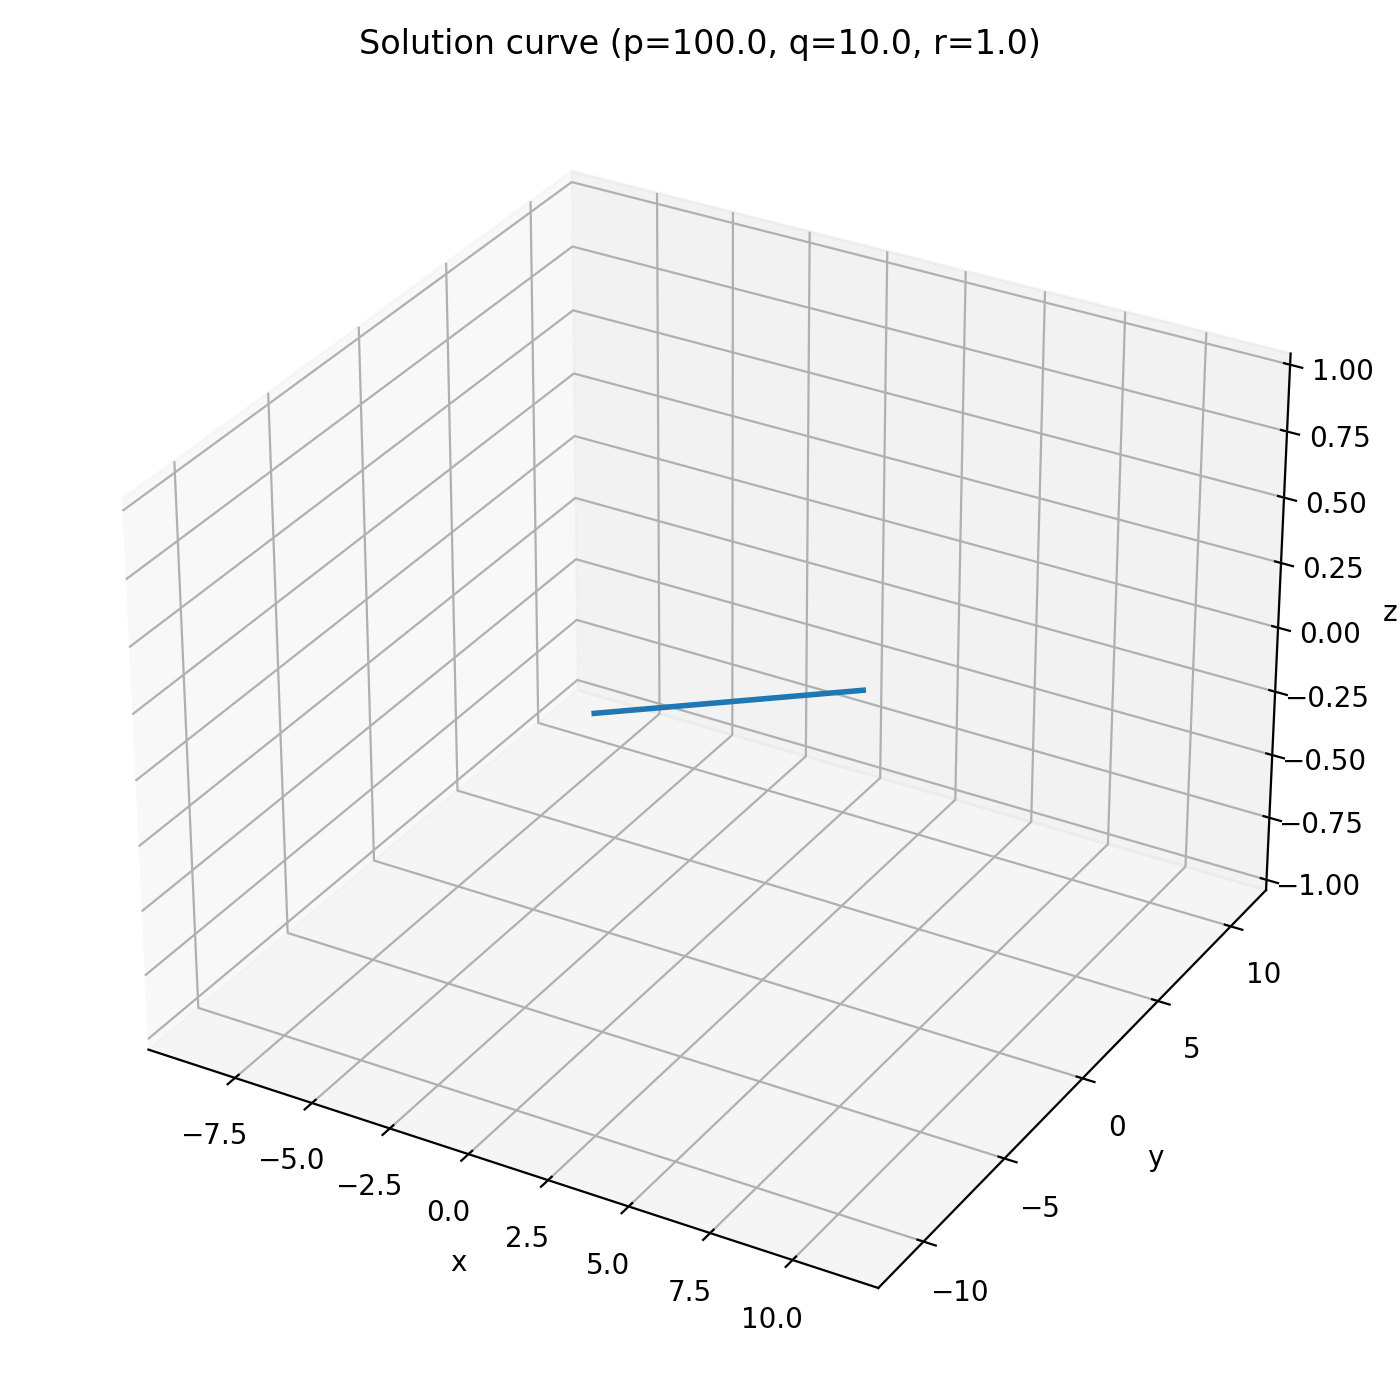
\includegraphics[width=0.7\columnwidth]{figs/hp_3d_only.png}
   \caption{}
   \label{}
   \end{figure}
\end{frame}

\begin{frame}[fragile]
    \frametitle{Code - C}
    \begin{lstlisting}

#include <stdio.h>
#include <math.h>
// Analyze the system: returns code (0=unique,1=no solution,2=infinitely many)
int analyze_system(double p, double q, double r, double *D_out, double *E_out){
double D = p*q - 11.0*p*r + 10.0*q*r;
double E = (p*r - 10.0*q*r) / 9.0;
if(D_out) *D_out = D;
if(E_out) *E_out = E;
const double tol = 1e-12;
if(fabs(D) > tol) return 0; // unique
if(fabs(E) > tol) return 1; // inconsistent
return 2; // infinitely many
}


    \end{lstlisting}
    \end{frame}

    \begin{frame}[fragile]
    \frametitle{Code - C}
    \begin{lstlisting}
// Parametric solution (only valid if analyze_system returns 2)
void parametric_solution(double t, double *x, double *y, double *z){
if(x) *x = 10.0 * t + 10.0/9.0;
if(y) *y = -11.0 * t - 1.0/9.0;
if(z) *z = t;
}


// Row reduction for 3x4 augmented matrix
void row_reduce_3x4(const double A_in[3][4], double A_out[3][4]){
int i,j;
for(i=0;i<3;i++){
for(j=0;j<4;j++){
A_out[i][j] = A_in[i][j];
}
}

\end{lstlisting}
\end{frame}

    \begin{frame}[fragile]
    \frametitle{Code - C}
    \begin{lstlisting}
// R2 <- R2 - 10 R1
for(j=0;j<4;j++){
A_out[1][j] -= 10.0 * A_out[0][j];
}
// R3 <- R3 - (qr) R1, qr = A_in[2][0]
double qr = A_in[2][0];
for(j=0;j<4;j++){
A_out[2][j] -= qr * A_out[0][j];
}
// s = (pr-qr)/90 ; pr = A_in[2][1]
double pr = A_in[2][1];
double s = (pr - qr) / 90.0;
for(j=0;j<4;j++){
A_out[2][j] -= s * A_out[1][j];
}
}

\end{lstlisting}
\end{frame}

\begin{frame}[fragile]
    \frametitle{Code - Python(with shared C code)}
    The code to obtain the required plot is
    \begin{lstlisting}
# plot_hp_3d.py
import ctypes
from ctypes import c_double, POINTER, byref
import numpy as np
import matplotlib.pyplot as plt
from mpl_toolkits.mplot3d import Axes3D  # noqa: F401 (needed for 3D projection)

# load shared library (libhp.so should be in current working directory)
lib = ctypes.CDLL("./libhp.so")

# bind functions
lib.analyze_system.argtypes = (c_double, c_double, c_double,
                               POINTER(c_double), POINTER(c_double))
lib.analyze_system.restype = ctypes.c_int

\end{lstlisting}
\end{frame}
\begin{frame}[fragile]
\frametitle{Code - Python(with shared C code)}
\begin{lstlisting}
lib.parametric_solution.argtypes = (c_double, POINTER(c_double),
                                    POINTER(c_double), POINTER(c_double))
lib.parametric_solution.restype = None

# row_reduce signature: void row_reduce_3x4(const double A_in[3][4], double A_out[3][4]);
lib.row_reduce_3x4.argtypes = (POINTER(c_double), POINTER(c_double))
lib.row_reduce_3x4.restype = None

# Python wrappers
def analyze(p, q, r):
    D = c_double(); E = c_double()
    code = lib.analyze_system(c_double(p), c_double(q), c_double(r),
                              byref(D), byref(E))
    return int(code), D.value, E.value
\end{lstlisting}
\end{frame}

\begin{frame}[fragile]
\frametitle{Code - Python(with shared C code)}
\begin{lstlisting}
def param_sol(t):
    x = c_double(); y = c_double(); z = c_double()
    lib.parametric_solution(c_double(t), byref(x), byref(y), byref(z))
    return x.value, y.value, z.value

def row_reduce(A):
    
    A = np.asarray(A, dtype=np.float64, order='C')
    if A.shape != (3,4):
        raise ValueError("A must be shape (3,4)")
    ArrayType = c_double * 12
    in_buf = ArrayType(*A.ravel().tolist())
    out_buf = ArrayType()
    lib.row_reduce_3x4(in_buf, out_buf)
    return np.frombuffer(out_buf, dtype=np.float64).reshape((3,4)).copy()


\end{lstlisting}
\end{frame}

\begin{frame}[fragile]
\frametitle{Code - Python(with shared C code)}
\begin{lstlisting}
# ---- Main demo ----
if __name__ == "__main__":
    # change these to test other triples
    p, q, r = 100.0, 10.0, 1.0

    # Build augmented matrix [M | b]
    A = np.array([
        [1.0,    1.0,    1.0,    1.0],
        [10.0, 100.0, 1000.0,    0.0],
        [q*r,   p*r,   p*q,      0.0]
    ], dtype=np.float64)

    # Call row reduction and show result
    A_red = row_reduce(A)
    print("Reduced augmented matrix (after specified elimination steps):")
    np.set_printoptions(precision=6, suppress=True)
    print(A_red)

\end{lstlisting}
\end{frame}

\begin{frame}[fragile]
\frametitle{Code - Python(with shared C code)}
\begin{lstlisting}
 # Analyze system
    code, D, E = analyze(p, q, r)
    print(f"analyze_system -> code={code}, D={D}, E={E}")
    # code: 0 = unique, 1 = no solution, 2 = infinitely many

    # If consistent (infinitely many), plot 3D solution curve
    if code == 2:
        ts = np.linspace(-1.0, 1.0, 401)
        xs = np.empty_like(ts); ys = np.empty_like(ts); zs = np.empty_like(ts)
        for i, t in enumerate(ts):
            xs[i], ys[i], zs[i] = param_sol(t)


\end{lstlisting}
\end{frame}

\begin{frame}[fragile]
\frametitle{Code - Python(with shared C code)}
\begin{lstlisting}
        fig = plt.figure(figsize=(7,7))
        ax = fig.add_subplot(111, projection='3d')
        ax.plot(xs, ys, zs, lw=2)
        ax.set_xlabel('x'); ax.set_ylabel('y'); ax.set_zlabel('z')
        ax.set_title(f'Solution curve (p={p}, q={q}, r={r})')
        plt.tight_layout()
        outname = "hp_3d_only.png"
        fig.savefig(outname, dpi=200)
        print("Saved 3D plot:", outname)
    else:
        print("System not consistent - nothing to plot.")

\end{lstlisting}
\end{frame}




\begin{frame}[fragile]
\frametitle{Code - Python only}
\begin{lstlisting}
import numpy as np
import matplotlib.pyplot as plt
from mpl_toolkits.mplot3d import Axes3D  # noqa: F401 (needed for 3D projection)

def row_reduce_3x4(A_in):
    A = np.asarray(A_in, dtype=float, order='C').copy()
    if A.shape != (3,4):
        raise ValueError("A_in must be shape (3,4)")
    # R2 <- R2 - 10 R1
    A[1,:] = A[1,:] - 10.0 * A[0,:]
    # R3 <- R3 - (qr) R1 (use qr from original A_in)
    qr = float(A_in[2,0])
    A[2,:] = A[2,:] - qr * A[0,:]
    # s = (pr - qr) / 90  (pr from original)


\end{lstlisting}
\end{frame}
\begin{frame}[fragile]
\frametitle{Code - Python only}
\begin{lstlisting}
    pr = float(A_in[2,1])
    s = (pr - qr) / 90.0
    A[2,:] = A[2,:] - s * A[1,:]
    return A

def analyze_system(p, q, r, tol=1e-12):
    D = p*q - 11.0*p*r + 10.0*q*r
    E = (p*r - 10.0*q*r) / 9.0
    if abs(D) > tol:
        return 0, D, E
    if abs(E) > tol:
        return 1, D, E
    return 2, D, E
\end{lstlisting}
\end{frame}

\begin{frame}[fragile]
\frametitle{Code - Python only}
\begin{lstlisting}
def parametric_solution(t):
    x = 10.0 * t + 10.0/9.0
    y = -11.0 * t - 1.0/9.0
    z = t
    return x, y, z

if __name__ == "__main__":
    # Choose (p,q,r). For consistent test use (100,10,1)
    p, q, r = 100.0, 10.0, 1.0

    # Build augmented matrix [M | b]
    A = np.array([
        [1.0,     1.0,    1.0,    1.0],
        [10.0,  100.0, 1000.0,    0.0],
        [q*r,   p*r,   p*q,       0.0]
    ], dtype=float)

\end{lstlisting}
\end{frame}

\begin{frame}[fragile]
\frametitle{Code - Python only}
\begin{lstlisting}
    print("Input augmented matrix [M | b]:")
    np.set_printoptions(precision=6, suppress=True)
    print(A)

    # Row-reduce with the exact steps used in math writeup
    A_red = row_reduce_3x4(A)
    print("\nReduced augmented matrix after specified elimination steps:")
    print(A_red)

    # Analyze with D,E
    code, D, E = analyze_system(p, q, r)
    status = {0: "unique solution (D != 0)", 1: "inconsistent (no solution)", 2: "infinitely many solutions"}
    print(f"\nanalyze_system -> code={code}, D={D:.6g}, E={E:.6g}  => {status[code]}")


\end{lstlisting}
\end{frame}

\begin{frame}[fragile]
\frametitle{Code - Python only}
\begin{lstlisting}
    # If consistent, plot only the 3D solution curve
    if code == 2:
        ts = np.linspace(-1.0, 1.0, 401)
        xs = np.empty_like(ts); ys = np.empty_like(ts); zs = np.empty_like(ts)
        for i,t in enumerate(ts):
            xs[i], ys[i], zs[i] = parametric_solution(t)

        fig = plt.figure(figsize=(7,7))
        ax = fig.add_subplot(111, projection='3d')
        ax.plot(xs, ys, zs, lw=2)
        ax.set_xlabel('x'); ax.set_ylabel('y'); ax.set_zlabel('z')
        ax.set_title(f'Solution curve (p={p}, q={q}, r={r})')
        plt.tight_layout()
        outname = "hp_3d_pure_python.png"
        fig.savefig(outname, dpi=200)
        print("\nSaved 3D plot:", outname)


\end{lstlisting}
\end{frame}

\begin{frame}[fragile]
\frametitle{Code - Python only}
\begin{lstlisting}
    else:
        print("\nSystem not consistent - nothing to plot.")



\end{lstlisting}
\end{frame}

\end{document}
